\documentclass[12pt]{article}
\usepackage[english]{babel}
\usepackage[utf8]{inputenc}

%% Pointer to 'default' preamble, other reusable files
% pacakages and definitions

\usepackage{geometry}
\geometry{
	letterpaper, 
	portrait, 
	top=.75in,
	left=.8in,
	right=.75in,
	bottom=.5in		} 	% Page Margins
	
%% additional packages for nice things
\usepackage{amsmath} 	% for most math
\usepackage{commath} 	% for abs
\usepackage{lastpage}	% for page count
\usepackage{amssymb} 	% for therefore
\usepackage{graphicx} 	% for image handling
\usepackage{wrapfig} 	% wrap figures
\usepackage[none]{hyphenat} % for no hyphenations
\usepackage{array} 		% for >{} column characterisctis
\usepackage{physics} 	% for easier derivative \dv....
\usepackage{tikz} 		% for graphic@!
\usepackage{circuitikz} % for circuits!
\usetikzlibrary{arrows.meta} % for loads
\usepackage[thicklines]{cancel}	% for cancels
\usepackage{xcolor}		% for color cancels
\usepackage[per-mode=fraction]{siunitx} % for si units and num
\sisetup{group-separator = {,}, group-minimum-digits = 3} % additional si unit table functionality

\usepackage{fancyhdr} 	% for header
\usepackage{comment}	% for ability to comment out large sections
\usepackage{multicol}	% for multiple columns using multicols
\usepackage[framed,numbered]{matlab-prettifier} % matlab sytle listing
\usepackage{marvosym} 	% for boltsymbol lightning
\usepackage{pdflscape} 	% for various landscape pages in portrait docs.
%\usepackage{float}
\usepackage{fancyvrb}	% for Verbatim (a tab respecting verbatim)
\usepackage{enumitem}	% for [resume] functionality of enumerate
\usepackage{spreadtab} 	% for using formulas in tables}
\usepackage{numprint}	% for number format in spread tab
\usepackage{subcaption} % for subfigures with captions
\usepackage[normalem]{ulem} % for strike through sout

% for row colors in tables....
\usepackage{color, colortbl}
\definecolor{G1}{gray}{0.9}
\definecolor{G2}{rgb}{1,0.88,1}%{gray}{0.6}
\definecolor{G3}{rgb}{0.88,1,1}

% For table formatting
\usepackage{booktabs}
\renewcommand{\arraystretch}{1.2}
\usepackage{floatrow}
\floatsetup[table]{capposition=top} % put table captions on top of tables

% Caption formating footnotesize ~ 10 pt in a 12 pt document
\usepackage[font={small}]{caption}

%% package config 
\sisetup{output-exponent-marker=\ensuremath{\mathrm{E}}} % for engineer E
\renewcommand{\CancelColor}{\color{red}}	% for color cancels
\lstset{aboveskip=2pt,belowskip=2pt} % for more compact table
%\arraycolsep=1.4pt\def
\setlength{\parindent}{0cm} % Remove indentation from paragraphs
\setlength{\columnsep}{0.5cm}
\lstset{
	style      = Matlab-editor,
	basicstyle = \ttfamily\footnotesize, % if you want to use Courier - not really used?
}
\renewcommand*{\pd}[3][]{\ensuremath{\dfrac{\partial^{#1} #2}{\partial #3}}} % for larger pd fracs
\renewcommand{\real}[1]{\mathbb{R}\left\{ #1 \right\}}	% for REAL symbol
\newcommand{\imag}[1]{\mathbb{I}\left\{ #1 \right\}}	% for IMAG symbol
\definecolor{m}{rgb}{1,0,1}	% for MATLAB matching magenta
	
%% custom macros
\newcommand\numberthis{\addtocounter{equation}{1}\tag{\theequation}} % for simple \numberthis command

\newcommand{\equal}{=} % so circuitikz can have an = in the labels
\newcolumntype{L}[1]{>{\raggedright\let\newline\\\arraybackslash\hspace{0pt}}m{#1}}
\newcolumntype{C}[1]{>{\centering\let\newline\\\arraybackslash\hspace{0pt}}m{#1}}
\newcolumntype{R}[1]{>{\raggedleft\let\newline\\\arraybackslash\hspace{0pt}}m{#1}}

%% Header
\pagestyle{fancy} % for header stuffs
\fancyhf{}
% spacing
\headheight 29 pt
\headsep 6 pt
%%% custom commands for nicer units
\newcommand{\mw}{\ensuremath{\text{ MW}}}
\newcommand{\hz}{\ensuremath{\text{ Hz}}}
\newcommand{\pu}{\ensuremath{\text{ Pu}}}
\newcommand{\sbase}{\ensuremath{\text{S}_{\text{Base}}}}
\newcommand{\fbase}{\ensuremath{f_{\text{Base}}}}
\newcommand{\mbase}[1]{\ensuremath{\text{M}_{\text{Base}_{#1}}}}
\newcommand{\hsys}{\ensuremath{\text{ H}_{\text{sys}}}}


%% Header
\rhead{Thad Haines \\ Page \thepage\ of \pageref{LastPage}}
\chead{Initial Six Machine Delay Scenario \\ 01-10-20}
\lhead{Research \\ }

%\usepackage{graphicx}
%\graphicspath{ {figures/} }
%\newcommand{\caseName}{ }

\begin{document}
\paragraph{Scenario: } 
Two area, six machine system loss of generation event. \\
% six machine system
\begin{figure}[!ht]
	\centering
	\footnotesize
	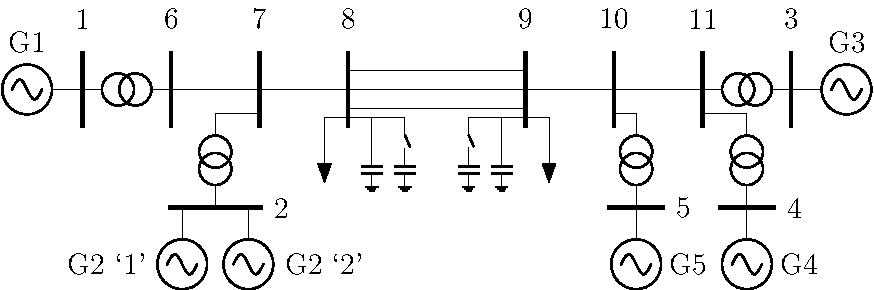
\includegraphics[width=.7\linewidth]{../../models/sixMachine/sixMachine}
	\caption{Six machine system.}
	\label{fig: six machine}
\end{figure}


Governed machines are: G1, G2 `1', G3, G4.\\
Governor time constants are identical for all machines and no deadbands are used.\\
PI filtered AGC signals are sent every 5 seconds to G1 and G3.\\

At t = 2, G2 `2', steps its mechanical power output $P_M$ down by 20\%.\\

All system settings are the same in test cases, with the exception of governor delays/filters on G3.\\
% tgov delay

\begin{figure}[!ht]
	\centering
	\footnotesize
	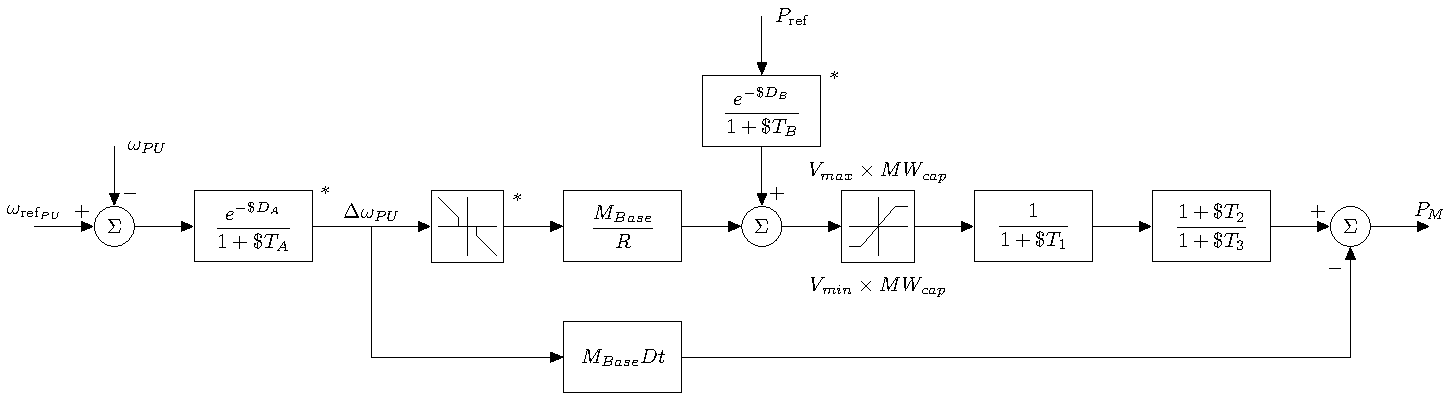
\includegraphics[width=\linewidth]{../../models/tgov1/tgov1DBdelay}
	\caption{Governor model with optional delays and deadbands indicated by a *.}
	\label{fig: modified tgov}
\end{figure}

Input $\Delta \omega_{PU}$ was delayed by 40 seconds and any changes to $P_{REF}$ were delayed by 10 seconds. \\
Low pass filtering of $\omega$ using a 30 second time constant was also tested.

\paragraph{Results:} The delayed governor response generates a second frequency perturbance 40 seconds after the first frequency event caused by the loss of generation.
The delay also introduces minor oscillations in frequency that are eventually damped out by other governor action.
Valve travel is increased by the delayed governor response.
However, the use of a lowpass filter can lessen frequency effects and actually reduce valve travel.

Regardless of filtering, the delay causes a larger frequency nadir.


\pagebreak

\newcommand{\caseName}{SixMachineDelayStep1}
\paragraph{Base Case Results:} \ \\
No Delay or filtering.
\\
\includegraphics[width=\linewidth]{figures/\caseName Freq}

\includegraphics[width=\linewidth]{figures/\caseName RACE}

\includegraphics[width=\linewidth]{figures/\caseName ValveTravel1}

\includegraphics[width=\linewidth]{figures/\caseName ValveTravel2}

\pagebreak
\renewcommand{\caseName}{SixMachineDelayStep3}
\paragraph{Delay Case Results: } \ \\
40 sec $\Delta \omega_{PU}$ delay, 10 sec $P_{ref}$ Delay.
\\
\includegraphics[width=\linewidth]{figures/\caseName Freq}

\includegraphics[width=\linewidth]{figures/\caseName RACE}

\includegraphics[width=\linewidth]{figures/\caseName ValveTravel1}

\includegraphics[width=\linewidth]{figures/\caseName ValveTravel2}


\pagebreak
\renewcommand{\caseName}{SixMachineDelayStep4}
\paragraph{Filtered Delay Case Results: } \ \\
40 sec $\Delta \omega_{PU}$ delay with a 30 sec low pass filter time constant, 10 sec  $P_{ref}$ Delay.
\\
\includegraphics[width=\linewidth]{figures/\caseName Freq}

\includegraphics[width=\linewidth]{figures/\caseName RACE}

\includegraphics[width=\linewidth]{figures/\caseName ValveTravel1}

\includegraphics[width=\linewidth]{figures/\caseName ValveTravel2}



%\paragraph{'Soft Goals':}
%	\begin{enumerate}
%	\item Write Thesis 2020
%	\end{enumerate}
		

\end{document}